\section{CUDA: copies vectorisées depuis la mémoire partagée}
\label{appendix:smem_vectorized}

Sur les GPUs NVIDIA, une seule copie peut faire jusqu'à 128bits de large.
Celà permet dans notre cas (implémentation d'un DGEMM) de copier deux doubles en une seule instruction.
Cependant, il faut que les deux doubles de la source soient contigus en mémoire partagée et qu'ils aillent tous deux dans des registres du même thread.

\begin{figure}[H]
    \centering
    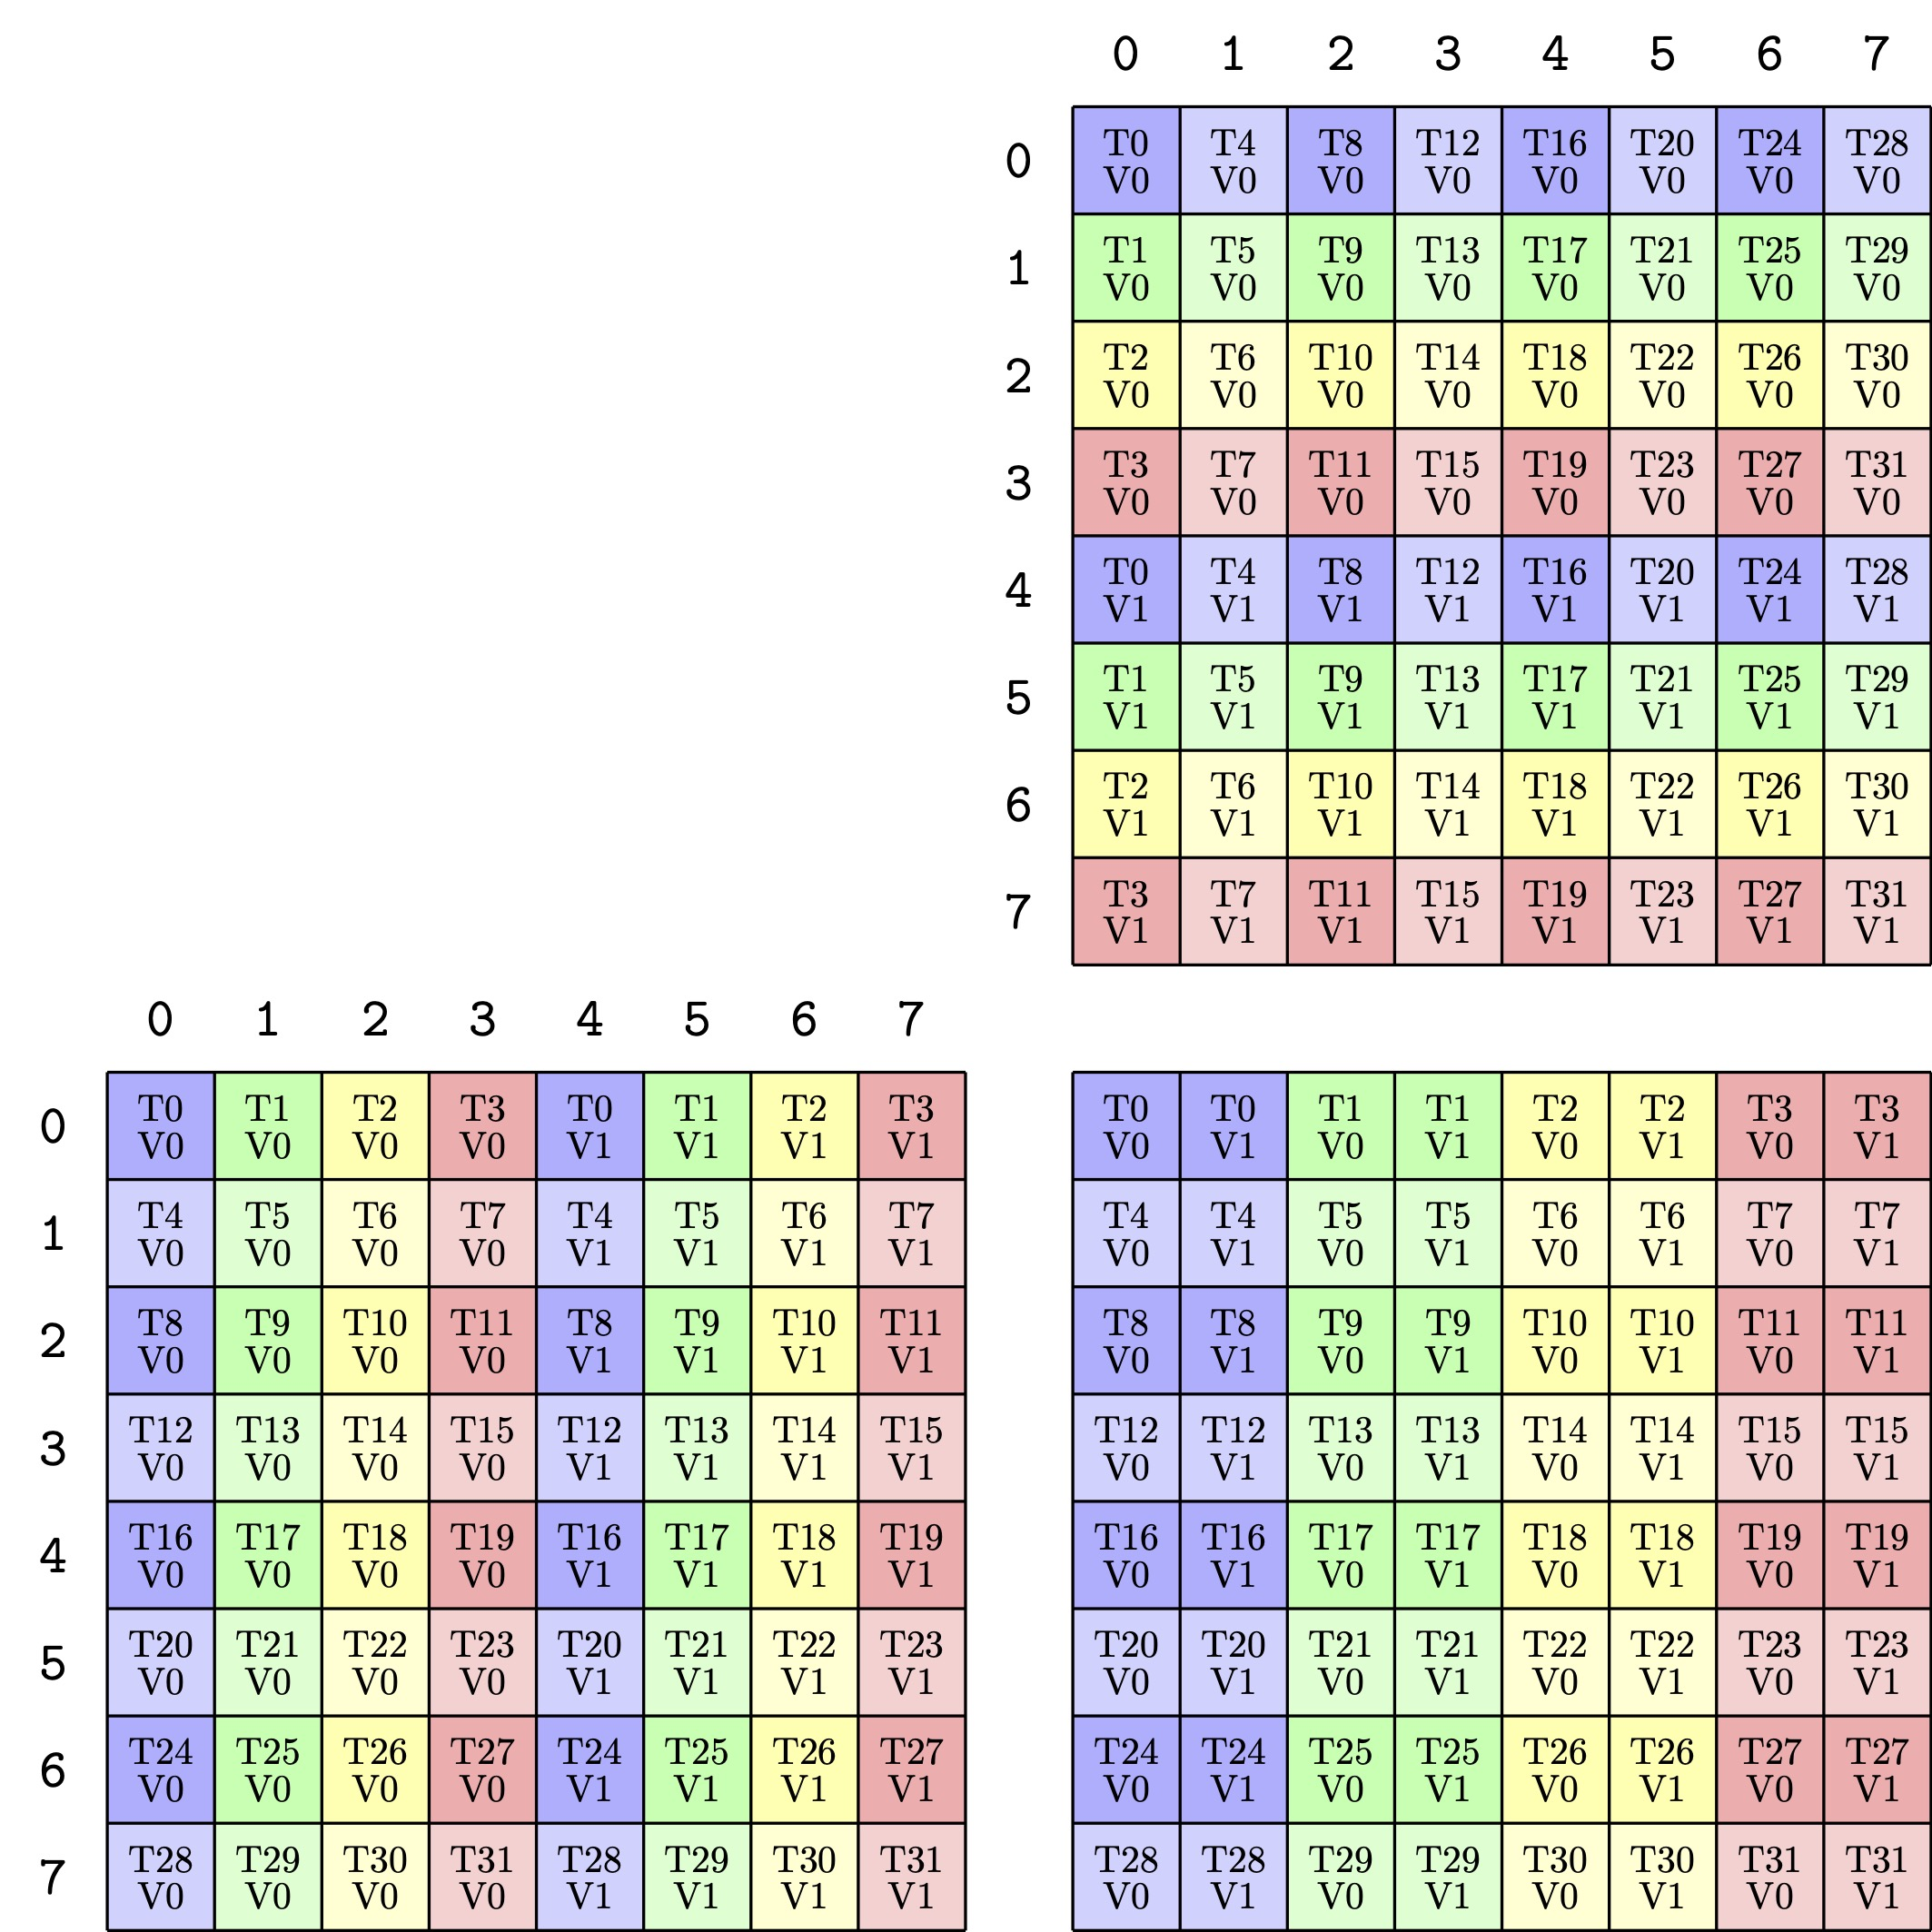
\includegraphics[width=1\textwidth]{assets/dgemm_cuda/m8n8k8.jpg}
    \caption{Schéma du partitionnement de A, B et C pour l'opération de tensor core double de Ampere.}
    \label{fig:m8n8k8_base}
\end{figure}

Sur la Figure \ref{fig:m8n8k8_base}, les valeurs 0 et 1 du thread 0 (T0V0 et T0V1) ne sont pas contigues en mémoire partagée.

\begin{figure}[H]
    \centering
    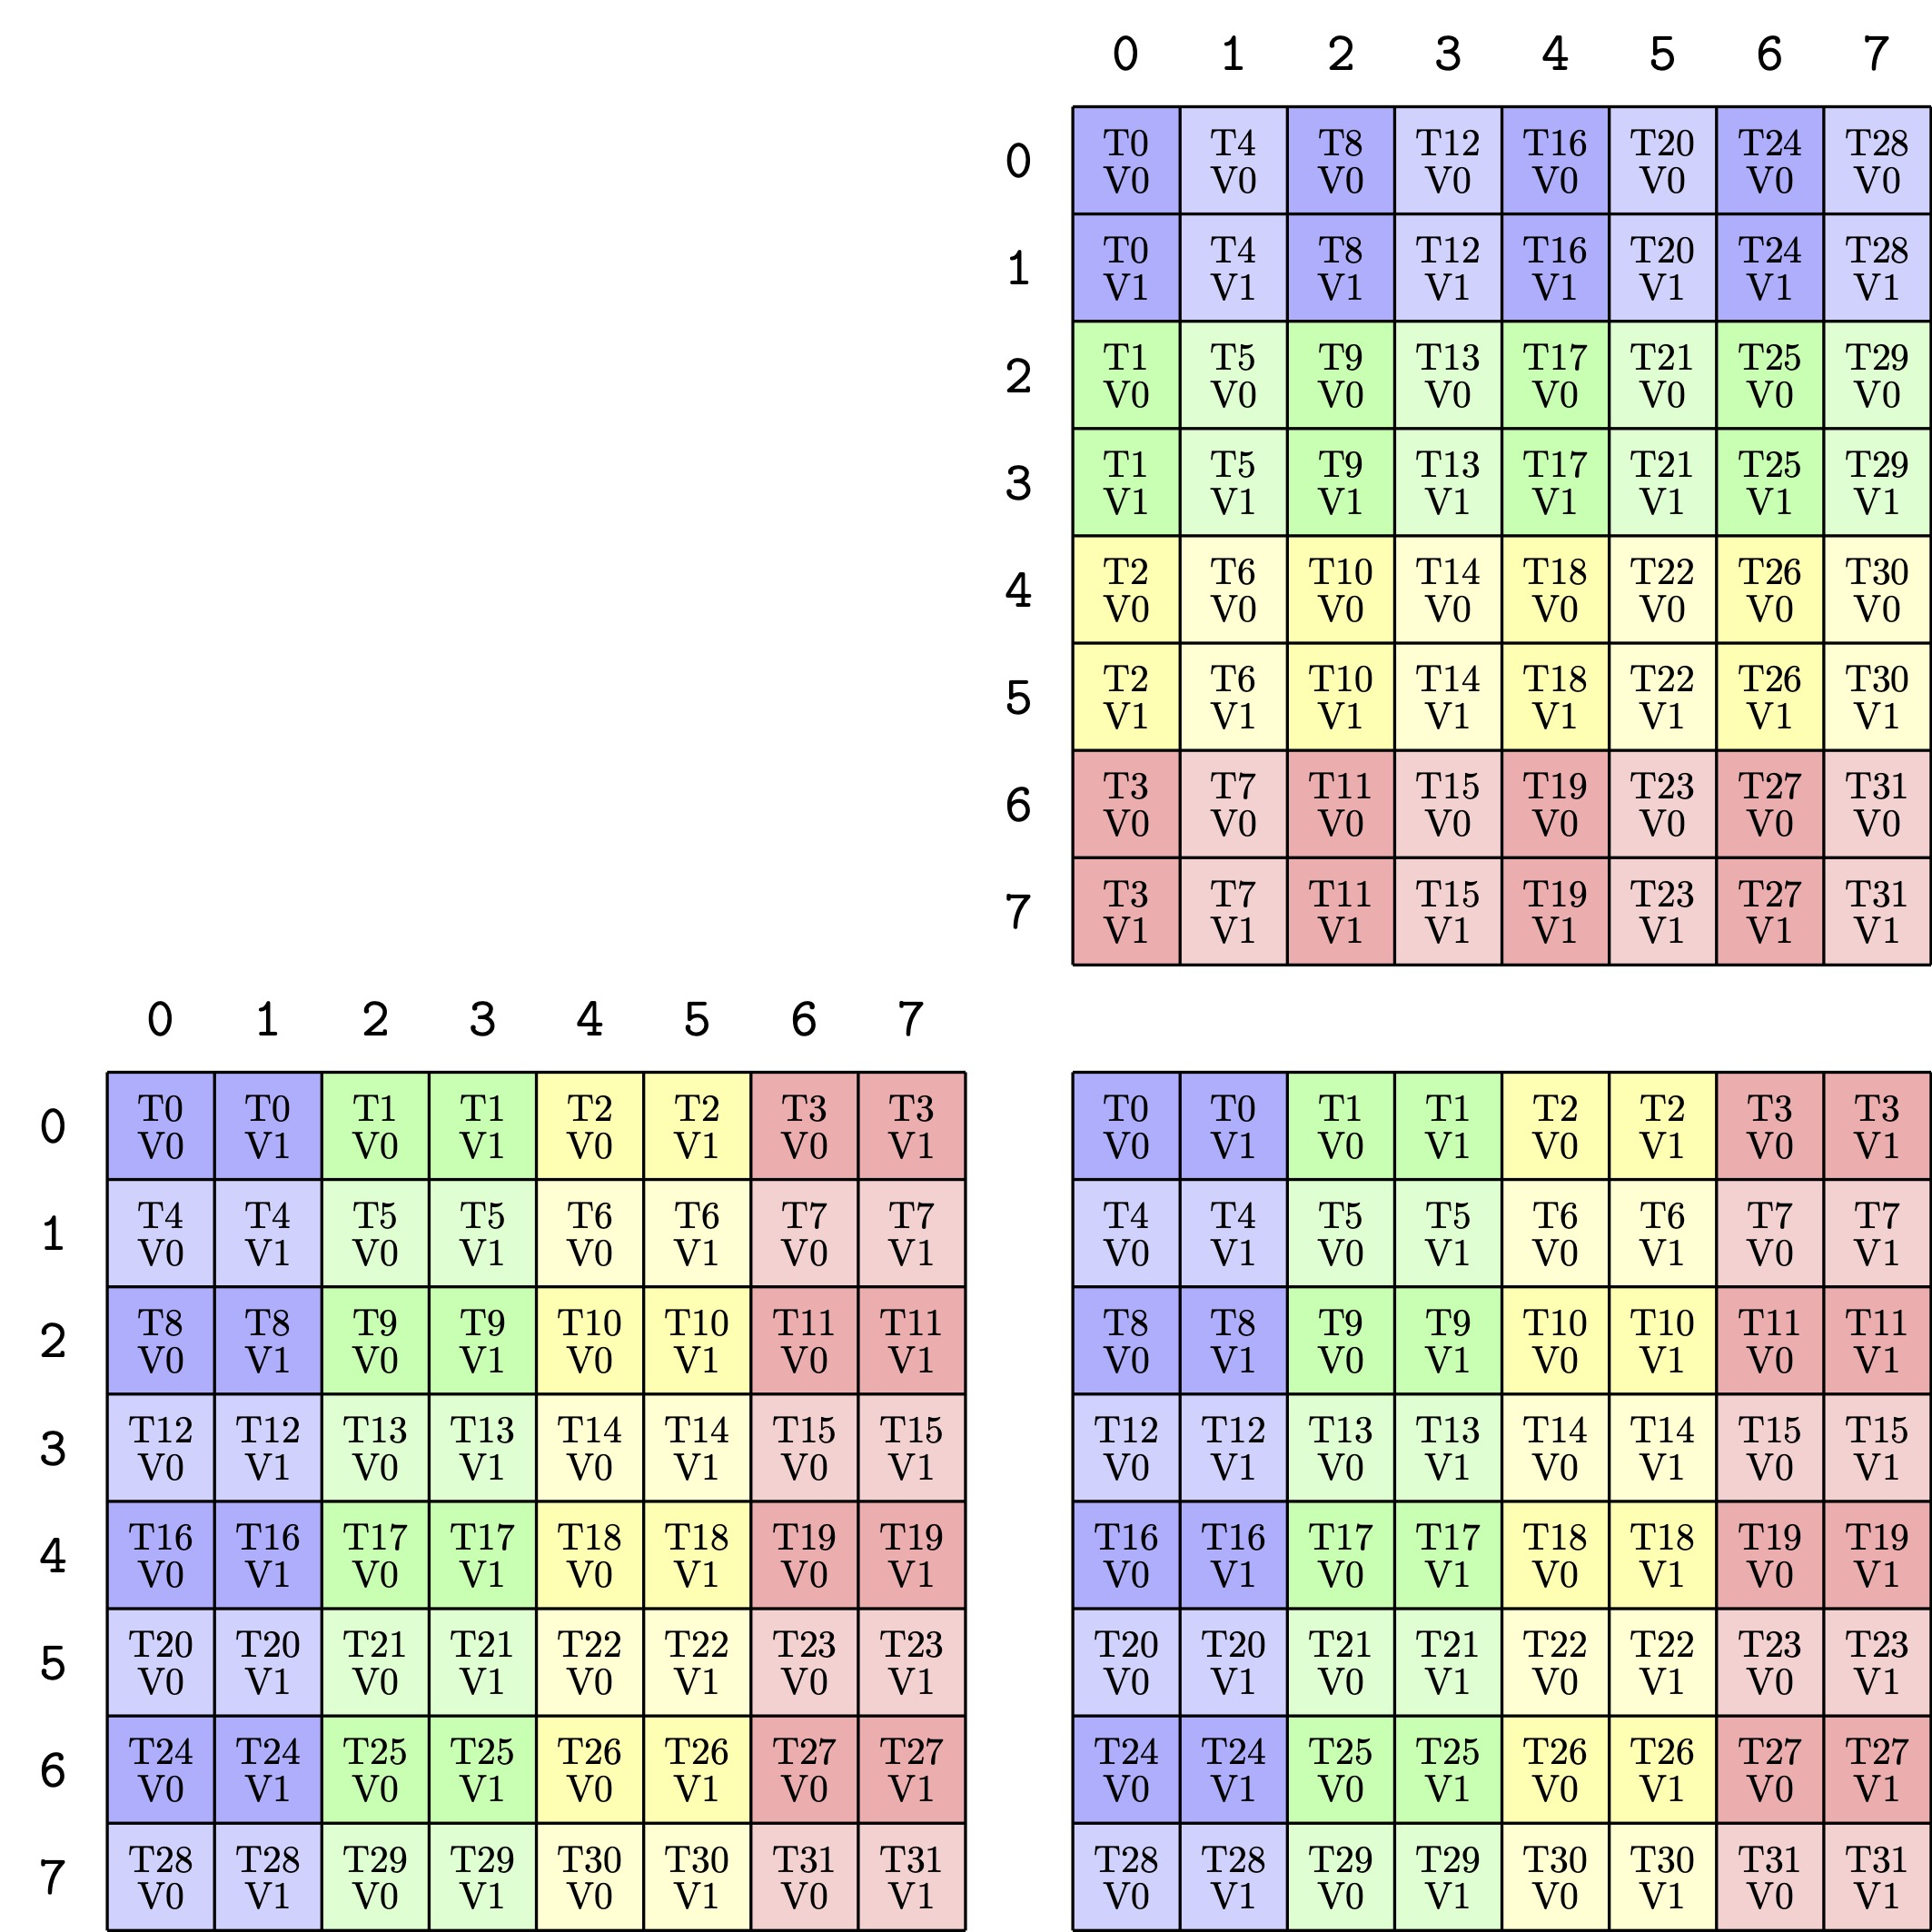
\includegraphics[width=1\textwidth]{assets/dgemm_cuda/m8n8k8_permuted.jpg}
    \caption{Schéma du partitionnement de A, B et C pour l'opération de tensor core double de Ampere (avec permutation du microkernel).}
    \label{fig:m8n8k8_permuted}
\end{figure}

Sur la version correctment permutée de ce microkernel (Figure \ref{fig:m8n8k8_permuted}), on voit que les valeurs 0 et 1 du thread 0 sont contigues en mémoire partagée (row-major), ils peuvent donc être chargés dans les 2 registres du thread 0 en une seule instruction de copie.

\section{CUDA: utilisation optimale des deux partitions du L2}
\label{appendix:l2split}

En 2021, des chercheurs de chez Citadel ont donné une présentation au GTC de NVIDIA\cite{gtc2021s33322} où ils ont montré qu'il existait une très grande pénalité de performance lors des accès à la "mauvaise" partie du L2 de la carte graphique depuis un SM.
Cette mauvaise partie est en fait la partition la plus loin du SM.
Les SMs sont disposés autour des deux partitions du L2 et lorsqu'ils veulent accéder à celle dont ils ne sont pas collés, ils doivent passer par l'interconnect des deux partitions du L2.

Ces chercheurs ont montré que la latence engendrée par un tel accès est 2x plus grande à la latence normale d'un accès au L2.

Nous avons reproduit\cite{leikoe2021ampere} ces benchmarks dans le cadre du projet (voir Figures \ref{fig:l2sm0} et \ref{fig:l2sm2}) en espérant pouvoir intégrer une optimisation en tirant partie à notre GEMM CUDA.
\begin{figure}[H]
    \centering
    \begin{minipage}{0.48\textwidth}
        \centering
        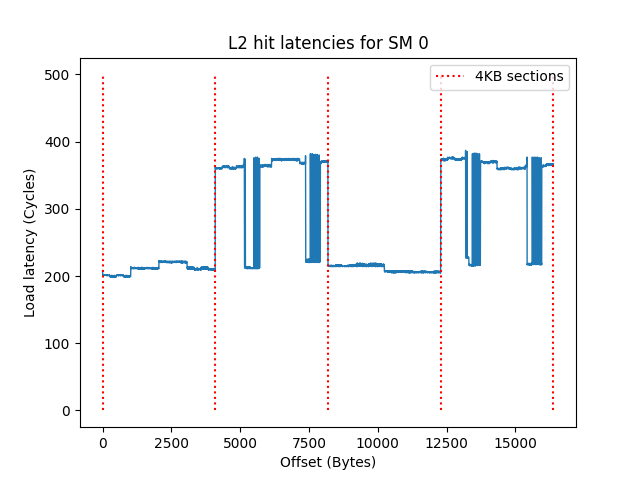
\includegraphics[width=\textwidth]{assets/dgemm_cuda/l2_latency_vs_offset_smid0.png}
        \caption{Graphique des latences engendrées par un accès en fonction de l'offset dans le L2 depuis le SM 0.}
        \label{fig:l2sm0}
    \end{minipage}
     \hfill
    \begin{minipage}{0.48\textwidth}
        \centering
        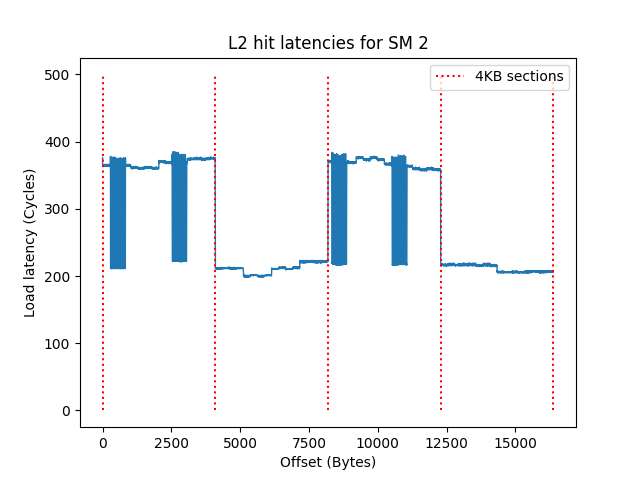
\includegraphics[width=\textwidth]{assets/dgemm_cuda/l2_latency_vs_offset_smid2.png}
        \caption{Graphique des latences engendrées par un accès en fonction de l'offset dans le L2 depuis le SM 1.}
        \label{fig:l2sm2}
    \end{minipage}
\end{figure}

Dans leur présentation, les chercheurs montrent que deux SMs consécutifs sont autour de la même partition puis que celà alterne.
Sur les Figures \ref{fig:l2sm0} et \ref{fig:l2sm2} on peut voir que le SM n°0 et le SM n°2 sont bien autour de deux partitions différentes.

La latence d'un accès à la partition proche du L2 est autour de 200 cycles alors qu'un accès accédant à l'autre partition coute plutôt 400 cycles.

Ils montrent sur leur benchmarks que un algorithme imaginé avec cette contrainte en tête peut gagner jusqu'à 85\% de performance par rapport au pire cas.
